\chapter{Gestion de la grille}\label{chap_grille}

La gestion de la grille et des bateaux est effectuée dans le module \texttt{bn\_grille.py}.

\section{La classe Bateau}
Cette classe, très minimaliste, définit un bateau par sa case de départ \texttt{Bateau.start}, sa taille \texttt{Bateau.taille} et sa direction \texttt{Bateau.sens}. Elle permet de récupérer :
\begin{itemize}
\item sa case de fin \texttt{Bateau.end},
\item la liste de ses cases occupées \texttt{Bateau.cases},
\item la liste de ses cases adjacentes \texttt{Bateau.cases\_adj}.
\end{itemize}

\section{La classe Grille}
\subsection{Présentation}
Cette classe est au c\oe ur du projet. Elle permet de mémoriser l'état de chaque case de la grille et d'effectuer des opérations comme :
\begin{itemize}
\item Gérer la liste des bateaux de la flotte : placer un bateau à une position donnée ou aléatoirement, placer une flotte aléatoire, supprimer un bateau coulé, ou encore garder la trace du plus grand bateau restant à couler.
\item Déterminer le nombre de cases vides autour d'une case donnée, dans chacune des directions.
\item Déterminer la liste, et le nombre, de bateaux possibles sur chaque case.
\item Déterminer lorsque la grille est terminée.
\end{itemize}
Beaucoup de ces fonctionnalités seront utilisées par l'algorithme de résolution.

\medskip

Afin de pouvoir faire évoluer les règles, elle prend les paramètres suivants lors de son initialisation :
\begin{itemize}
\item \texttt{xmax} et \texttt{ymax} : les dimensions de la grille
\item \texttt{taille\_bateaux} : la liste des bateaux
\end{itemize}
\medskip

Dans la mesure où la grille a deux utilisations différentes (la grille du joueur et la grille de suivi des coups), j'ai d'abord décidé de créer deux classes héritées de \texttt{Grille} lors de la conception du projet, \texttt{GrilleJoueur(Grille)} et \texttt{GrilleSuivi(Grille)}, afin de distinguer leurs méthodes spécifiques. Après coup je me suis rendu compte que cela n'apportait pas d'avantage significatif en terme de qualité de code donc je ne les utiliserai pas, mais elles sont encore présentes dans mon code pour une évolution future du projet.

\subsection{État de la grille}

L'attribut \texttt{Grille.etat} fournit l'état de la grille. C'est un dictionnaire indexé par les tuples \texttt{(0,0)}, \texttt{(0,1)},... , \texttt{(9,9)}, dans lesquels la première coordonnée correspond à la colonne de la case et la deuxième à sa ligne.\\
L'état d'une case peut être :
\begin{itemize}
\item $0$ : case vide
\item $1$ : case touchée (ou contenant un bateau)
\item $-1$ : case manquée ou impossible
\end{itemize}
%L'intérêt d'utiliser un dictionnaire plutôt qu'une liste double tient au fait que les appels sont plus simples et plus naturels et, surtout, que l'utilisation d'une table de hachage permet la recherche d'un élément en $O(1)$.  

\medskip

La méthode \texttt{Grille.test\_case(self, case)} permet de déterminer si une case est valide et vide, et \texttt{Grille.is\_touche(self, case)} indique si une case donnée contient ou non un bateau.

\medskip

Notons également l'utilisation de l'attribut \texttt{Grille.vides} qui est la liste des cases vides. Bien entendu, cette classe contient une fonction \texttt{Grille.update(self)} de mise à jour jour de l'état de la grille (liste des cases vides, tailles du plus petit et du plus grand bateau restant).

\medskip

Enfin, la méthode \texttt{Grille.adjacent(self, case)} renvoie la liste de cases adjacentes à une case donnée.

\subsection{Gestion des espaces vides}
La méthodes \texttt{Grille.get\_max\_space(self, case, direction, face=True)} renvoie le nombre de cases vides dans une direction donnée. Grâce aux constantes de direction, un seul calcul est nécessaire pour englober tous les cas (horizontal et vertical). L'algorithme est donné en annexe \ref{algo_liste}, page \pageref{get_max_space}.
%\begin{algo1}
%direction[0]\sto dh\\
%direction[1]\sto dv\\
%0\sto m\\
%case[0]\sto x\\
%case[1]\sto y\\
%Tant que la case (x+dh, y+dv) est vide et est dans la grille :\\
%\tab{1} m+1\sto m\\
%\tab{1} x+dh\sto x\\
%\tab{1} y+dv\sto y\\
%Retourner m\\
%\end{algo1}

Si le paramètre \texttt{face==True}, la détermination se fait dans les deux sens (espace libre total horizontal ou vertical).

\medskip

La méthode \texttt{Grille.elimine\_cases(self)} parcourt toutes les cases vides et élimine celles dans lesquelles le plus petit bateau ne peut pas rentrer en mettant leur état à \texttt{-1}.

\subsection{Liste des bateaux possibles sur chaque case}
La méthode \texttt{Grille.get\_possibles(self)} renvoie d'une part la liste des bateaux possibles démarrant sur chaque case (ainsi que leurs directions) et, d'autre part, la liste des positions (et directions) de départ possibles pour chaque bateau. Pour ce faire on procède en deux temps :
\begin{itemize}
\item Dans un premier temps, on parcourt la liste des cases vides et pour chacune de ces cases on détermine, pour chaque bateau et chaque direction (droite et bas), s'il peut démarrer sur cette case. Cela fournit le dictionnaire \texttt{Grille.possibles\_cases} indexé par les cases et dont les éléments sont une liste de tuples de la forme \texttt{(taille, direction)}.\\
Par exemple : \texttt{\{(0,0):[(5,(1,0)), (5,(0,1)),...], (0,1):...\}}
\item Dans un deuxième temps, on "retourne" ce dictionnaire pour obtenir le dictionnaire \texttt{Grille.possibles} indexé par les tailles des bateaux et dont les éléments sont une liste de tuples de la forme \texttt{(case, direction)}.\\
Par exemple : \texttt{\{5:[((0,0), (1,0)), ((0,0), (0,1)), ((1,0), (1,0)),...], 4:...\}}
\end{itemize}

\medskip

Cette méthode va servir à faire plusieurs choses :
\begin{itemize}
\item Créer une flotte aléatoire grâce au dictionnaire \texttt{Grille.possibles}, dans la méthode \texttt{Grille.init\_bateaux\_alea(self)}.
\item Déterminer la case optimale dans l'algorithme de résolution au niveau 5.
\item Optimiser la file d'attente dans les algorithmes de résolution.
\item Déterminer tous les arrangements possibles de bateaux sur la grille.
\end{itemize}

L'algorithme complet de cette méthode est donné en annexe \ref{algo_liste}, page \pageref{get_possibles}.

% -------------------------------------------------------------
\begin{comment}
\subsection{Nombre de possibilités sur chaque case}
L'une des parties importantes de l'algorithme de résolution consiste en la détermination de la case dans laquelle rentrent le plus de bateaux. Cette question intervient lors de la phase de tirs en aveugle et, lorsqu'on a touché une première case, qu'on doit tester ses cases adjacentes (phase de tir ciblé).
\subsubsection{Optimisation de la phase de tir en aveugle}\label{opti_aveugle}
La méthode \texttt{Grille.case\_max(self)} renvoie la case vide contenant le plus de bateaux, ainsi que le nombre de bateaux qu'elle contient. L'algorithme est très simple : d'abord on crée un dictionnaire \texttt{Grille.probas} indexé par les cases et contenant le nombre de bateaux possibles grâce à \texttt{Grille.possibles}. Ensuite il ne reste plus qu'à renvoyer celle qui en contient le plus.

\subsubsection{Optimisation de la phase de tir ciblé}\label{opti_touche}
Cette optimisation est un petit peu plus délicate. Une fois qu'une case a été touchée, l'algorithme va tester ses 4 (au maximum) cases adjacentes et les ranger en ordre décroissant du nombre de bateaux possibles. C'est le rôle de la méthode \texttt{Grille.case\_max\_touchee(self, case\_touchee)}. 

Notons \texttt{(x, y)} les coordonnées de la case touchée et intéressons nous au nombre de bateaux possibles sur les cases adjacentes horizontales (pour les verticales, c'est exactement la même chose). Pour chaque taille de bateau à couler possible contenant \texttt{case\_touchee} il faudra distinguer trois cas :
\begin{enumerate}
\item Le bateau est à gauche de \texttt{case\_touchee} et se termine sur cette case. Dans ce cas on augmente de 1 le nombre de possibilités de la case à gauche \texttt{(x-1, y)}
\item Le bateau est à cheval sur \texttt{case\_touchee}. Dans ce cas on augmente de 1 le nombre de possibilités de la case à gauche \texttt{(x-1, y)} et de celle à droite \texttt{(x+1, y)}
\item Le bateau est à droite de \texttt{case\_touchee} et commence sur cette case. Dans ce cas on augmente de 1 le nombre de possibilités de la case à droite \texttt{(x+1, y)}
\end{enumerate}

\textbf{Exemple :}

Imaginons que, sur une grille vierge, on vienne de toucher la case de coordonnées $(5,0)$ et regardons le nombre de façons de placer le bateau de taille 4 à gauche et à droite :
\begin{enumerate}
\item Le bateau rentre à gauche de la case $(5,0)$ :

\begin{center}
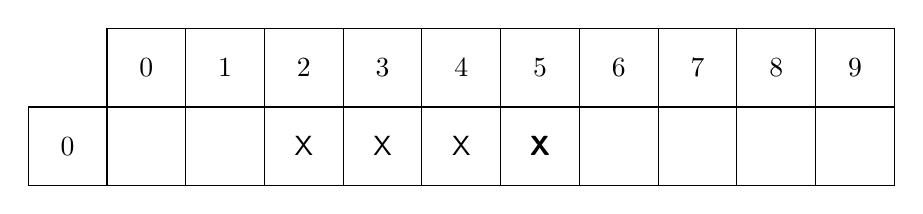
\begin{tikzpicture}
\draw (0,1)--(10,1);
\draw (-1,0)--(10,0);
\draw (-1,-1)--(10,-1);
\foreach \x in {0,1,...,10}{
\draw (\x,1)--(\x,-1);
}
\draw (-1,0)--(-1,-1);
\foreach \x in {0,1,...,9}{
\draw (\x+0.5,0.5) node{\x};
}
\draw (-0.5, -0.5) node{$0$};
\draw (5.5, -0.5) node{\textbf{\textsf{X}}};

\draw (2.5, -0.5) node{\textsf{X}};
\draw (3.5, -0.5) node{\textsf{X}};
\draw (4.5, -0.5) node{\textsf{X}};
\end{tikzpicture}\\
\textit{La case $(4,0)$ est augmentée de 1
}\end{center}

\item Le bateau est à cheval sur la case $(5,0)$ (2 possibilités) :
\begin{center}

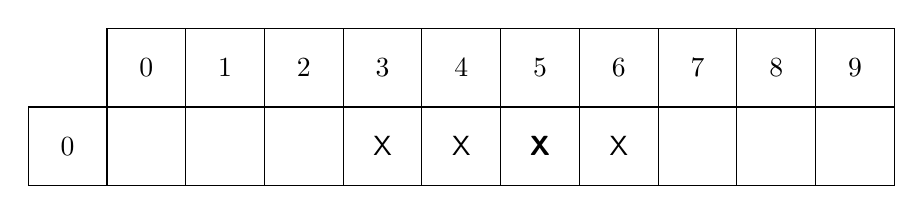
\begin{tikzpicture}
\draw (0,1)--(10,1);
\draw (-1,0)--(10,0);
\draw (-1,-1)--(10,-1);
\foreach \x in {0,1,...,10}{
\draw (\x,1)--(\x,-1);
}
\draw (-1,0)--(-1,-1);
\foreach \x in {0,1,...,9}{
\draw (\x+0.5,0.5) node{\x};
}
\draw (-0.5, -0.5) node{$0$};
\draw (5.5, -0.5) node{\textbf{\textsf{X}}};

\draw (6.5, -0.5) node{\textsf{X}};
\draw (3.5, -0.5) node{\textsf{X}};
\draw (4.5, -0.5) node{\textsf{X}};
\end{tikzpicture}
%\textit{Les cases $(4,0)$ et $(6,0)$ sont augmentées de 1
%}\end{center}
%
%\begin{center}

\medskip

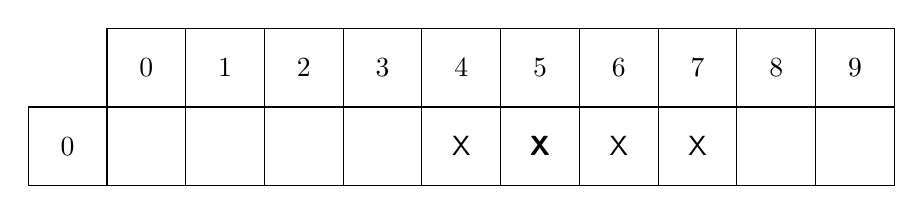
\begin{tikzpicture}
\draw (0,1)--(10,1);
\draw (-1,0)--(10,0);
\draw (-1,-1)--(10,-1);
\foreach \x in {0,1,...,10}{
\draw (\x,1)--(\x,-1);
}
\draw (-1,0)--(-1,-1);
\foreach \x in {0,1,...,9}{
\draw (\x+0.5,0.5) node{\x};
}
\draw (-0.5, -0.5) node{$0$};
\draw (5.5, -0.5) node{\textbf{\textsf{X}}};

\draw (6.5, -0.5) node{\textsf{X}};
\draw (7.5, -0.5) node{\textsf{X}};
\draw (4.5, -0.5) node{\textsf{X}};
\end{tikzpicture}\\
\textit{Les cases $(4,0)$ et $(6,0)$ sont augmentées de 2
}\end{center}

\item Le bateau rentre à droite de la case $(5,0)$ :

\begin{center}
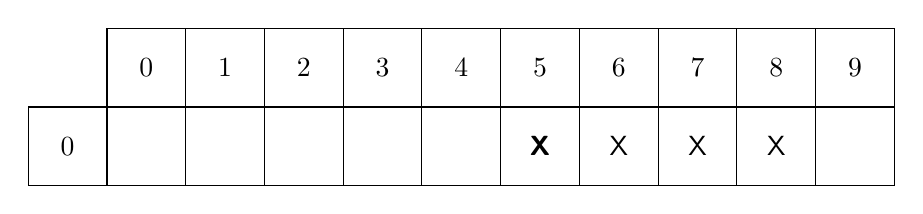
\begin{tikzpicture}
\draw (0,1)--(10,1);
\draw (-1,0)--(10,0);
\draw (-1,-1)--(10,-1);
\foreach \x in {0,1,...,10}{
\draw (\x,1)--(\x,-1);
}
\draw (-1,0)--(-1,-1);
\foreach \x in {0,1,...,9}{
\draw (\x+0.5,0.5) node{\x};
}
\draw (-0.5, -0.5) node{$0$};
\draw (5.5, -0.5) node{\textbf{\textsf{X}}};

\draw (6.5, -0.5) node{\textsf{X}};
\draw (7.5, -0.5) node{\textsf{X}};
\draw (8.5, -0.5) node{\textsf{X}};
\end{tikzpicture}\\
\textit{La case $(6,0)$ est augmentée de 1
}\end{center}
\end{enumerate} 
Au final, la case $(4,0)$ admet 3 bateaux horizontaux de taille 4 et idem pour la case $(6,0)$.

Si la case $(3,0)$ avait été jouée et manquée nous aurions obtenu 1 bateau horizontal de taille 4 possible sur la case $(4,0)$ et 2 sur la case $(6,0)$ :

\begin{center}
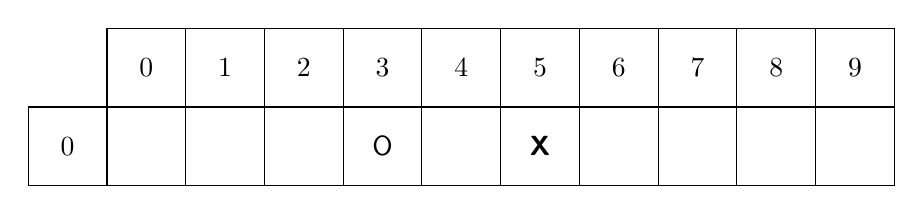
\begin{tikzpicture}
\draw (0,1)--(10,1);
\draw (-1,0)--(10,0);
\draw (-1,-1)--(10,-1);
\foreach \x in {0,1,...,10}{
\draw (\x,1)--(\x,-1);
}
\draw (-1,0)--(-1,-1);
\foreach \x in {0,1,...,9}{
\draw (\x+0.5,0.5) node{\x};
}
\draw (-0.5, -0.5) node{$0$};
\draw (5.5, -0.5) node{\textbf{\textsf{X}}};

\draw (3.5, -0.5) node{\textsf{O}};
\end{tikzpicture}\\
\end{center}

Une fois que le compte des bateaux possibles a été effectué sur chacune des cases adjacentes, on crée une liste \texttt{probas\_liste} contenant des tuples de la forme \texttt{(case, probas[case])} que l'on ordonne en ordre décroissant de possibilités grâce à l'instruction \texttt{sorted(probas\_liste, key=lambda proba: proba[1], reverse = True)} et que l'on retourne.

\end{comment}
% -------------------------------------------------------------


\subsection{Gestion de la flotte}
Le classe \texttt{Grille} contient toutes les méthodes nécessaires pour gérer la flotte de bateaux. Les méthodes \texttt{Grille.get\_taille\_max(self)} et \texttt{Grille.get\_taille\_min(self)} mettent à jour respectivement la taille maximum et la taille minimum des bateaux restant à trouver. La méthode \texttt{Grille.rem\_bateau(self, taille)} permet de supprimer de la liste \texttt{Grille.taille\_bateaux} un bateau coulé.

\subsubsection{Ajout d'un bateau}
La méthode \texttt{Grille.add\_bateau(self, bateau)} permet d'ajouter un bateau (instance de la classe \texttt{Bateau}) après avoir testé sa validité via la méthode \texttt{Grille.test\_bateau(self, bateau)}, et marque ses cases adjacentes comme impossibles.

\subsubsection{Création d'un flotte aléatoire}
La méthode \texttt{Grille.add\_bateau\_alea(self, taille)} permet d'ajouter un bateau aléatoire de taille donnée sur la grille.

Pour créer une flotte aléatoire, on utilise la méthode \texttt{Grille.init\_bateaux\_alea(self)} dont l'algorithme est donné en annexe \ref{algo_liste}, page \pageref{init_alea}.

%\begin{algo1}
%0\sto nb\_bateaux\\
%Tant que nb\_bateaux < nombre de bateaux à placer :\\
%\tab{1} 0\sto nb\_bateaux\\
%\tab{1} On crée une copie temporaire de la grille dans gtmp\\
%\tab{1} Pour chaque taille de bateau à placer :\\
%\tab{2} On récupère les positions possibles pour ce bateau dans gtmp\\
%\tab{2} Si aucune possibilité :\\
%\tab{3} On casse la boucle et on recommence tout\\
%\tab{4} (pour éviter une situation de blocage)\\
%\tab{2} Sinon :\\
%\tab{3} On choisit une position et une direction au hasard\\
%\tab{4} (parmi celles possibles)\\
%\tab{3} On ajoute le bateau à gtmp\\
%\tab{3} nb\_bateaux+1\sto nb\_bateaux\\
%Enfin on copie l'état de gtmp dans notre grille \\
%\end{algo1}

\subsection{Fin de la partie}
L'attribut \texttt{Grille.somme\_taille}, initialisé dès le départ avec la classe \texttt{Grille}, contient le nombre total de cases à toucher. La méthode \texttt{Grille.fini(self)} compare donc ce nombre avec le nombre de cases touchée dans \texttt{Grille.etat} pour déterminer si la grille a été résolue.